\documentclass[../../main.tex]{subfiles}

\begin{document}
\problem{33}
\begin{wts}
What languages does your browser accept for response?
\end{wts}
\begin{proof}
\begin{wts}
    The baseband signal $x(t)$ has a bandwidth of $10$kHz and a peak-to-average power ratio of $\frac{x^2_max}{P_x}=3$. It is converted into a digital signal using the Nyquist sampling rate and a uniform quantizer.
    \begin{enumalpha}
        \item What is the signal-to-quantization-noise power ratio (SNR) if its bit rate is $120$ kbps?
        \item What is the necessary bit rate to achieve a signal-to-quantization-noise power ratio (SNR) of $48$db?
    \end{enumalpha}
\end{wts}
\begin{proof}[Proof of Part A]
    Let $b$ denote the number of bits per sample, and $R_b$ be the effective bitrate.
    \[f_{nyquist}\times b = R_b = 120\pow{3}\mathrm{Hz}\]
    Since $f_{nyquist}=2\times 10\pow{3}$Hz, and $b=6$ follows immediately. Write the step size $\Delta$
    \begin{equation}\label{step size uncertainty}
    \Delta = \begin{cases}\dfrac{2\norm{x}_u}{2^b-1}&\text{or}\\[3ex]
    \dfrac{2\norm{x}_u}{2^b}
    \end{cases}
    \end{equation}
    and
    \[SNR =\begin{cases} \dfrac{12P_x(2^b-1)^2}{4\norm{x}_u^2}=3969&\text{or}\\[3ex]
    \dfrac{12P_x(2^b)^2}{4\norm{x}_u}=4096
    \end{cases}\]
    The case for when $SNR$ is given in decibels follows immediately, one simply has to apply
    \begin{equation}\label{decibel conversion}
    SNR_db = 10\log_{10}\biggl(SNR\biggr)
    \end{equation}
\end{proof}
\begin{proof}[Proof of Part B]
    It is clear from Equation \eqref{decibel conversion} that 
    \[10^{4.8}=\dfrac{P_x}{\sigma_{eq}^2}\]
    After some trivial calculations, of which we will omit and using Equation \eqref{step size uncertainty} the effective bitrate $R_b$ is hence given by
    \[R_b=\begin{cases}\log_2\biggl\{\sqrt{10^{4.8}}+1\biggr\}\cdot 20\pow{3}\\
    \log_2\biggl\{\sqrt{10^{4.8}}\biggr\}\cdot 20\pow{3}\end{cases}\]
\end{proof}
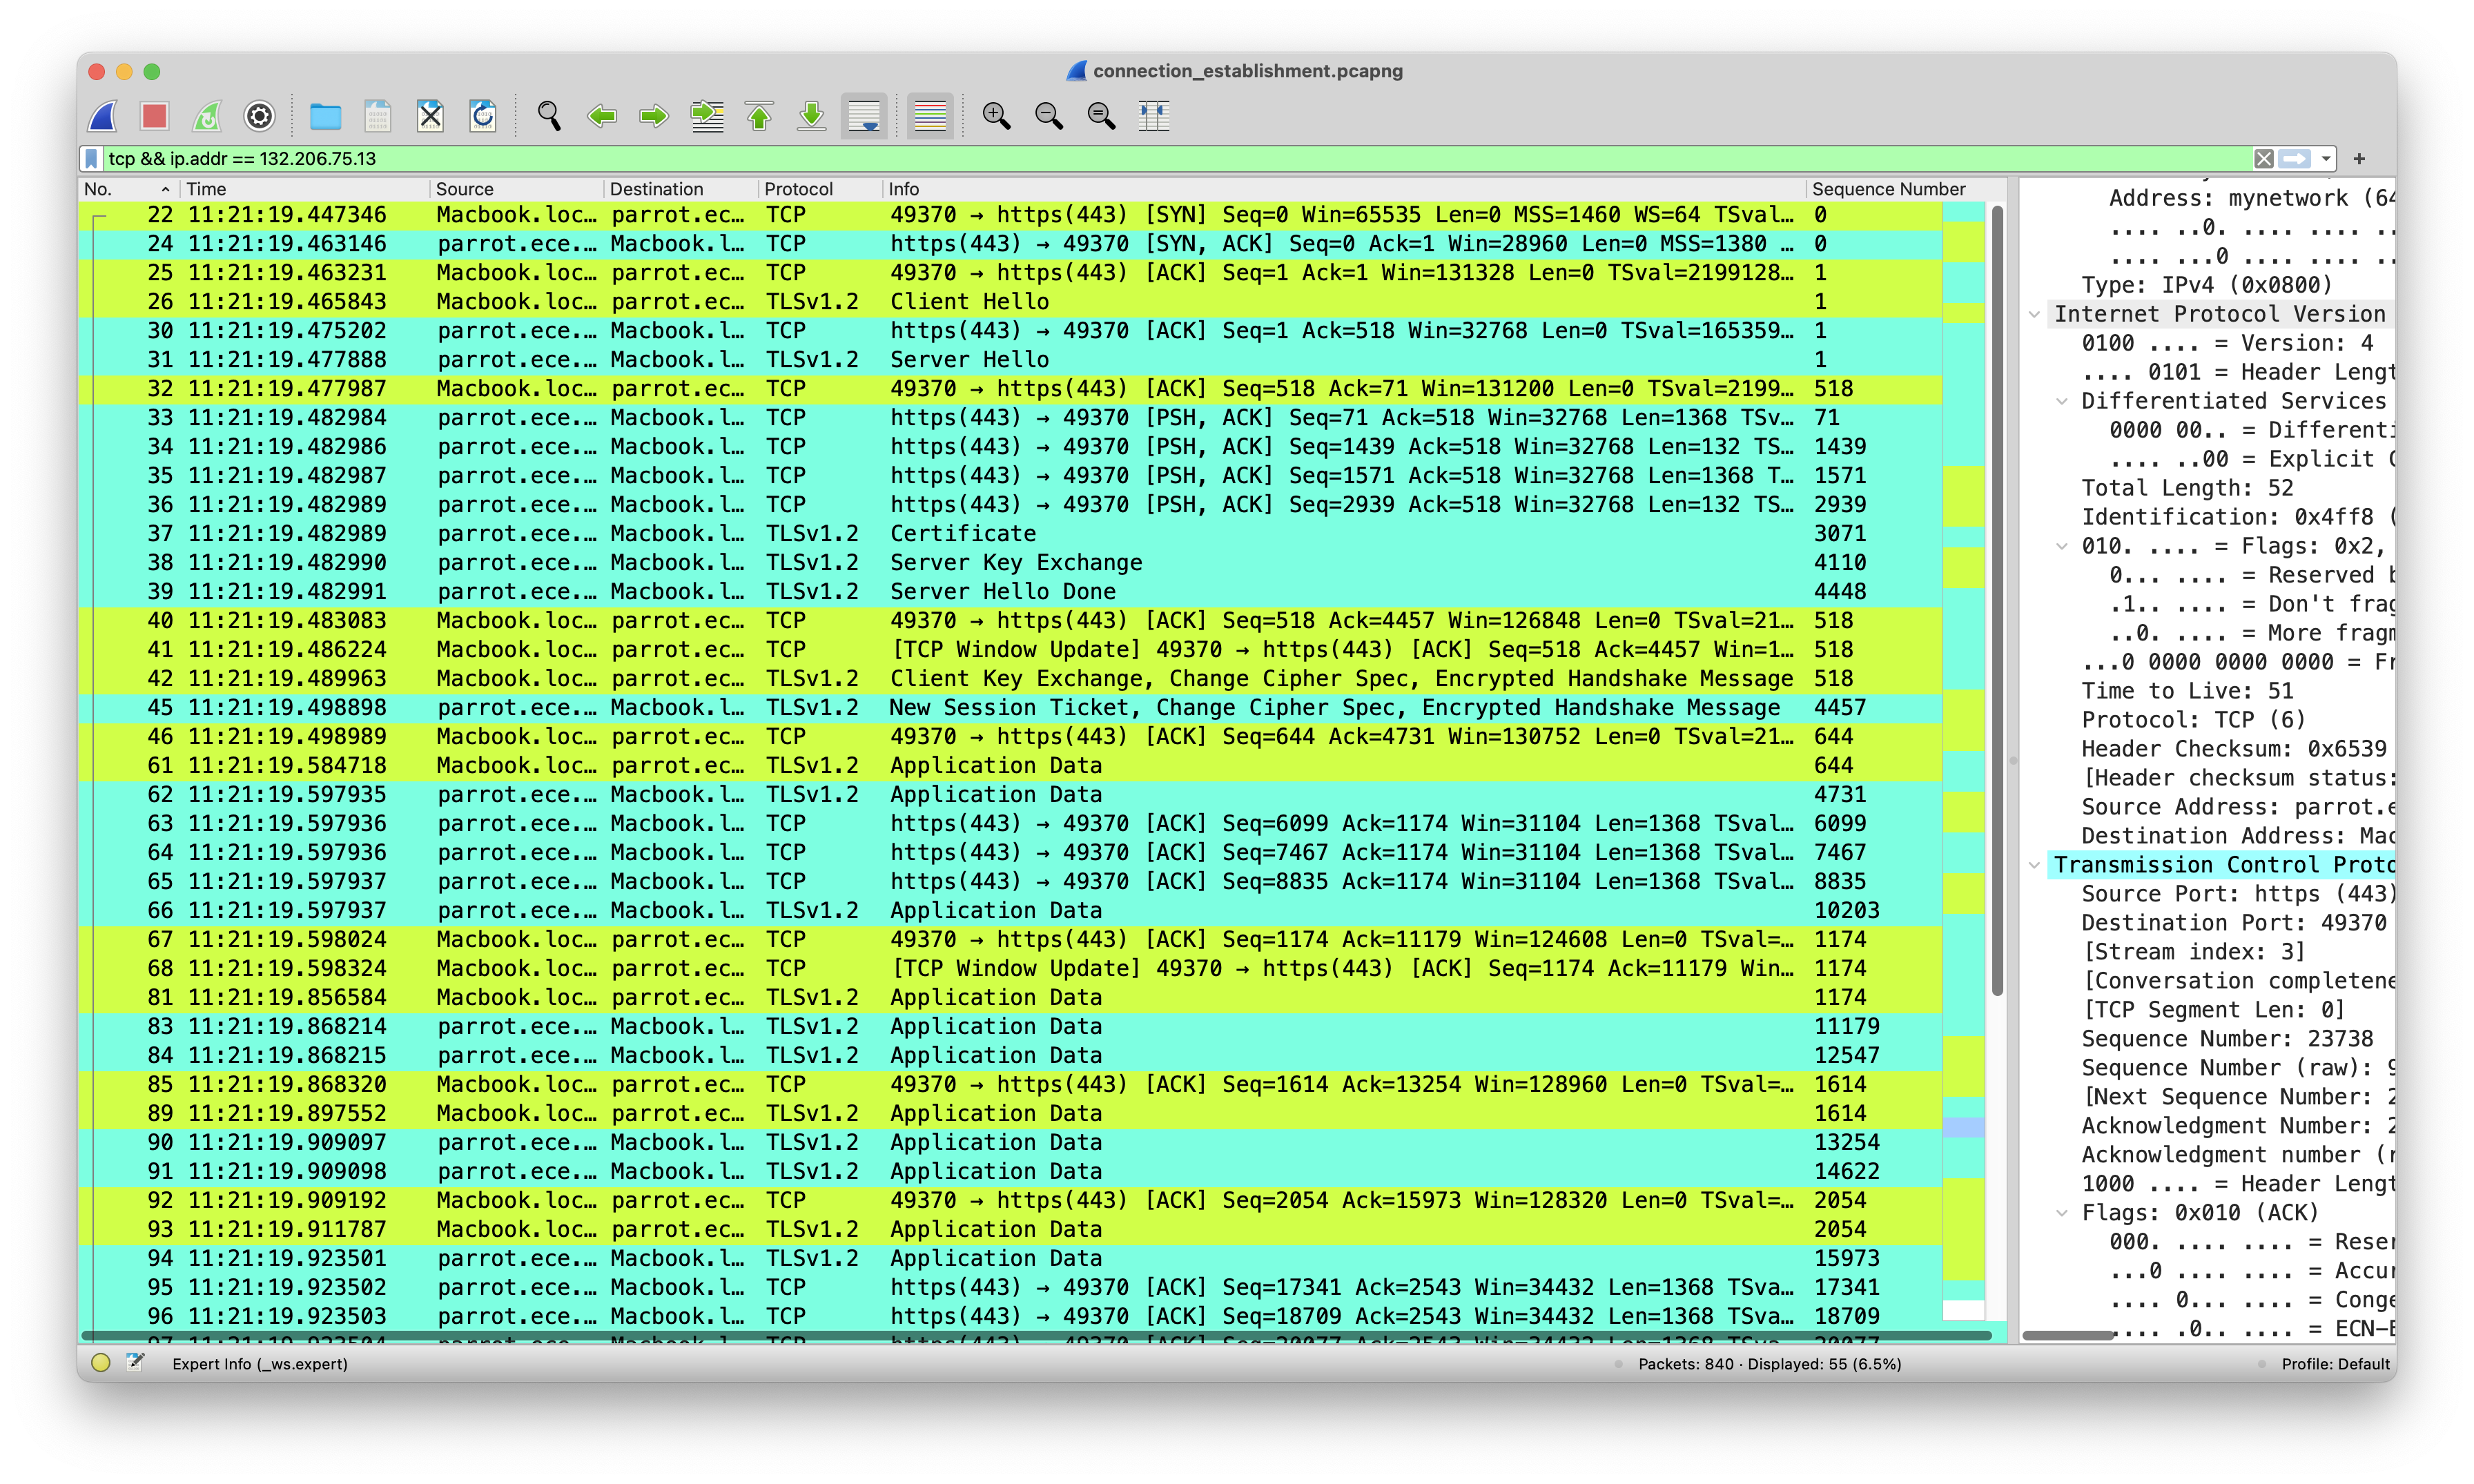
\includegraphics[width=\textwidth]{subfiles/images/L4N1_PAGE15_LIST_OF_PACKETS_1.png}
\end{proof}

\end{document}